\documentclass[a4paper]{article}

  \usepackage{fullpage} % Package to use full page
  \usepackage{parskip} % Package to tweak paragraph skipping
  \usepackage{tikz} % Package for drawing
  \usepackage{amsmath}
  \usepackage{siunitx} % Package for scientific units
  \usepackage{amsfonts}
  \usepackage{amssymb}
  \usepackage{hyperref}
  \usepackage[utf8]{inputenc}
  \usepackage[english]{babel}
  \usepackage{multicol}
  \usepackage{graphicx} % Package for including images
  \graphicspath{ {./images/} }
  
  \newcommand\tab[1][0.5cm]{\hspace*{#1}}
  
  \title{Assignment 1}
  \author{Adrian Darian}
  \date{9/4/2020}
  
  \begin{document}
  
\maketitle
  
\section*{Chapter 1}
\begin{itemize}
	\item[6] There are approximately $260$ million passenger vehicles registered in the United States. Assume that the battery in the average vehicle stores $540$ watt-hours ($\si{\watt\hour}$) of energy. Estimate (in gigawatt-hours) the total energy stored in US passenger vehicles. \\
	      \begin{tabular}{r c l}
	      	$w_{total}$ & $=$ & $nw_{avg}$                    \\
	      	            & $=$ & $(260,000,000)(540)$          \\
	      	            & $=$ & $140,400,000,000$             \\
	      	            & $=$ & $\SI{140.4}{\giga\watt\hour}$ \\
	      \end{tabular} 
	\item[11] The current at the terminals of the element is \\
	      \hbox to 2cm{}
	      \tab\begin{tabular}{l c}
	      $i = 0$, & $t < 0$ \\
	      $i = 40te^{-500t}\si{\ampere}$, & $t \geq 0$
	\end{tabular}
	\begin{itemize}
		\item[a)] Find the expression for the charge accumulating at the upper terminal. \\
		      \begin{tabular}{r c l}
		      	$q(t)$ & $=$ & $40\int_{0}^t te^{-500t}dt$                                                           \\
		      	       & $=$ & $40[(t(\frac{e^{-500t}}{-500}))_{0}^t - [\int_{0}^t \frac{e^{-500t}}{-500}dt]]$       \\
		      	       & $=$ & $40[(t(\frac{e^{-500t}}{-500}))_{0}^t + \frac{1}{500}(\frac{e^{-500t}}{-500})_{0}^t]$ \\
		      	       & $=$ & $\frac{40}{(500)^2}[(-500te^{-500t})_{0}^t - (e^{-500t})_{0}^t]$                      \\
		      	       & $=$ & $0.16[1-(500t + 1)e^{-500t}]\si{\milli\coulomb}$                                      \\
		      \end{tabular}
		\item[b)] Find the charge that has accumulated at $t = \SI{1}{\ms}$. \\
		      \begin{tabular}{r c l}
		      	$q(t)$ & $=$ &   
		      \end{tabular}
	\end{itemize}
	\item[12] When a car has a dead battery, it can often be started by connecting the battery from another car across its terminals. The positive terminals are connected together as are the negative terminals. The connection is illustrated in Fig. P1.12. Assume the current $i$ in Fig. P1.12 is measured and found to be $40$ \si{\ampere}.\\
	      \hbox to 2cm{} \\
	      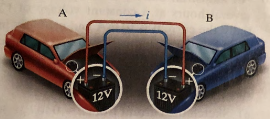
\includegraphics{P1-12.png} \\
	      \begin{itemize}
	      	\item[a)] Which car has the dead battery?
	      	\item[b)] If this connection is maintained for $1.5 \si{\min}$, how much energy is transferred to the dead battery? 
	      \end{itemize}
	\item[18] The voltage and current at the terminals of the circuit element if Fig 1.5 are zero for $t < 0$. For $t \geq 0$ they are \\
	      \hbox to 2cm{}
	      \tab\begin{tabular}{l}
	      $v = 75 - 75e^{-1000t}\si{\volt}$ \\
	      $i = 50e^{-1000t}\si{\milli\ampere}$
	\end{tabular}
	\begin{itemize}
		\item[a)] Find the maximum value of the power delivered to the circuit. \\
		      \begin{tabular}{l c c}
		      	$p(t)$ & $=$ & $vi$ \\
		      	       & $=$ &      \\
		      	       & $=$ &      \\
		      	       & $=$ &      \\
		      	       & $=$ &      \\
		      	       & $=$ &      \\
		      	       & $=$ &      \\
		      \end{tabular}
		\item[b)] Find the total energy delivered to the element. \\
		      \begin{tabular}{l c c}
		      	$p(t)$ & $=$ & $vi$ \\
		      	       & $=$ &      \\
		      	       & $=$ &      \\
		      	       & $=$ &      \\
		      	       & $=$ &      \\
		      	       & $=$ &      \\
		      	       & $=$ &      \\
		      \end{tabular} 
	\end{itemize}
	\item[27] The voltage and the current at the terminals of an automobile battery during a charge cycle are shown in Fig.P1.27.
	      \begin{itemize}
	      	\item[a)] Calculate the total charge transferred to the battery. \\
	      	      \begin{tabular}{r c l}
	      	      	$q$ & $=$ & area under $i$ vs $t$ plot                                    \\
	      	      	    & $=$ & $\frac{1}{2}(8)(12000) + (16)(12000) + \frac{1}{2}(16)(4000)$ \\
	      	      	    & $=$ & $\SI{272,000}{\coulomb}$                                      \\
	      	      \end{tabular}
	      	\item[b)] Calculate the total energy transferred to the battery. \\
	      	      \begin{tabular}{r c l}
	      	      	$W$                                         & $=$ & $\int pdt = \int vidt$                                                      \\
	      	      	For $0 \leq t \leq \SI{12,000}{\sec}$:      &     &                                                                             \\
	      	      	$v$                                         & $=$ & $250\times10^{-6}t + 8$                                                     \\
	      	      	$i$                                         & $=$ & $24 - 666.67\times10^{-6}t$                                                 \\
	      	      	$p$                                         & $=$ & $192 + 666.67\times10^{-6}t - 166.67\times10^{-9}t^{2}$                     \\
	      	      	$W_{1}$                                     & $=$ & $\int_{0}^{12,000} (192 + 666.67\times10^{-6}t - 166.67\times10^{-9}t^2)dt$ \\
	      	      	$W_{1}$                                     & $=$ & $\SI{2256}{\kilo\joule}$                                                    \\
	      	      	For $12,000 \leq t \leq \SI{16,000}{\sec}$: &     &                                                                             \\
	      	      	$v$                                         & $=$ & $250\times10^{-6}t + 8$                                                     \\
	      	      	$i$                                         & $=$ & $64 - 4\times10^{-3}t$                                                      \\
	      	      	$p$                                         & $=$ & $512 - 16\times10^{-3}t - \times10^{-6}t^{2}$                               \\
	      	      	$W_{2}$                                     & $=$ & $\int_{12,000}^{16,000} (512 - 16\times10^{-3}t - \times10^{-6}t^{2})dt$    \\
	      	      	$W_{2}$                                     & $=$ & $\SI{2256}{\kilo\joule}$                                                    \\
	      	      	$W_{T}$                                     & $=$ & $2256 + 362.667 = \SI{2618.667}{\kilo\joule}$                               \\
	      	      \end{tabular} 
	      \end{itemize}
	      % \begin{tikzpicture}[domain=0:20]
	      	      	      	      	      	      	      	      	      	      	      	      	      	      	      	      	      	      	      	      	      	      	      	      	      	      	      	      
	      % \end{tikzpicture}
	\item[33] Assume you are an engineer in charge of a project and one of your subordinate engineers reports that the interconnection in Fig.P1.33 does not pass the power check. The data for the interconnection are given in Table P1.33. \\
	      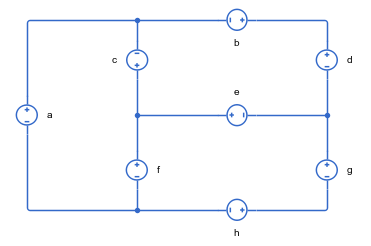
\includegraphics{P1-33.png} \\
	      \begin{tabular}{l c c c}
	      	Element & Voltage (\si{\volt}) & Current (\si{\ampere}) & Power ($\si{\volt}\times\si{\ampere} = \si{\watt}$) \\
	      	a       & 900                  & -22.5                  & -20250                                              \\
	      	b       & 105                  & -52.5                  & 5512.5                                              \\
	      	c       & -600                 & -30.0                  & -18000                                              \\
	      	d       & 585                  & -52.5                  & -30712.5                                            \\
	      	e       & -120                 & 30.0                   & 3600                                                \\
	      	f       & 300                  & 60.0                   & 18000                                               \\
	      	g       & 585                  & 82.5                   & -48262.5                                            \\
	      	h       & -165                 & 82.5                   & 13612.5                                             \\
	      	Total   & 1590                 & 97.5                   & -3600                                               
	      \end{tabular}	  
	      \begin{itemize}
	      	\item[a)] Is the subordinate correct? Explain your answer. \\
	      	      The subordinate is correct, due the net power being $\SI{-3600}{\watt}s$ and interconnection must consume power for each atom.
	      	\item[b)] If the subordinate is correct, can you find the error in the data?  \\
	      	      Elements c, d, and g supply extra power. To fix we just reduce the power to match the required load of the system.
	      \end{itemize} 
	      	      	      	      	      	      	      	      	      	      	      	      	      	      	      
\end{itemize}

  
\end{document}